\chapter{研究流域与数据}
\label{chap:data_and_All_Global_Stations}

\section{研究流域}

本论文各章节采用的研究流域均基于全球径流数据库(Global Runoff Data Base, GRDB),全球径流指数和元数据存档(Global Streamflow Indices and Metadata Archive, GSIM)以及补充的中国流域径流数据221个三部分共同组成。其中,搜集的中国流域的数据目的在于补充全球数据集中在中国记录缺失的空白。

\subsection{全球径流数据集}

全球径流数据库是由世界气象组织(World Meteorological Organization, WMO)于20世纪80年代组织建立的国际数据档案库,其中保存着长达200年的数据,旨在促进促进跨国和全球的水文数据和信息交换,帮助地球科学领域的学者分析全球气候趋势并评估环境影响和风险。GRDB提供的观测径流数据已经被广泛应用于国家、地区和全球尺度的水文分析、模型开发及评估等研究中\cite{burekUseGRDCGauging2023, houGlobalEvaluationRunoff2023}。\par
全球径流数据库最初建立在20世纪80年代初收集的初始数据集上,这些数据集是为了响应世界气象组织的要求,由成员国提供的全球水文数据,以补充第一次全球GARP试验(First Global GARP Experiment, FGGE)框架内的特定大气数据。这些数据集最初包含了1980年前后几年的月尺度径流数据,后来又纳入了联合国教科文组织1965-1985年的月尺度径流数据。在世界气象组织的支持下,经过三十多年的数据收集和质量控制,历史平均每日和每月径流的数据库得以稳步增长,最早的数据可以追溯到1806年,而最新的数据则是近实时更新的。目前,该数据库涵盖了来自全球159个国家和地区的10829个观测站点的每日和每月河流流量时间序列数据,总计约470,000个站点年,平均记录长度为45年,最长纪录长度为217年。数据库中所有的径流观测数据均公开下载(\href{https://grdc.bafg.de/GRDC/EN/02_srvcs/21_tmsrs/210_prtl/prtl_node.html}{https://grdc.bafg.de/GRDC/EN/02\_srvcs/21\_tmsrs/210\_prtl/prtl\_node.html},最后访问时间:2024年7月29日)。\par
此外,GRDB还根据其收集的数据生成各种数据产品,例如长期统计数据和年度特征分析,以及流入世界海洋的表面淡水通量。中心还提供了许多GIS图层,包括各个站点的集水区边界,便于生成地图产品。这些资源大大促进了全球水文和气候研究,使研究人员能够更好地理解和应对全球变化带来的挑战。径流观测站位置如图\ref{fig:All_Global_Stations}(a)所示。\par

GSIM由Do等人创建\cite{doGlobalStreamflowIndices2018, gudmundssonGlobalStreamflowIndices2018},是来自世界各地的每日河流流量现场观测的综合集合,旨在加强对大尺度淡水资源的了解。作为GRDB的扩展,GSIM档案整合包括欧洲径流档案(European Water Archive, EWA),俄罗斯区域水文数据网络(A Regional, Electronic, Hydrographic Data Network for Russia, ARCTICNET),中国水文数据项目(China Hydrology Database Project, CHDP),美国国家水信息系统(US National Water Information System, USGS)等在内的12个不同来源的数据,并对数据进行了广泛、正式而标准的数据质量控制流程,最终形成了包含30,959个独特的站点的元数据的数据集(\href{https://doi.pangaea.de/10.1594/PANGAEA.887470}{https://doi.pangaea.de/10.1594/PANGAEA.887470},最后访问时间:2024年8月2日)。\par
GSIM数据集包括各种类型的元数据,如站点id、地理坐标、站点海拔、径流指数和集水区边界等。基于观测站的日径流数据,计算出月度、季度和年度三种时间分辨率的流量属性,以及年最大最小值(MAX, MIN)、平均值(MEAN)、第10个百分位数(P10)、中位数(P50)、第90个百分位数(P90)等多种径流指数。基于全球数字高程模型(Digital Elevation Model,DEM)和重新定位算法提取了流域边界,使得用户可以轻松的提取感兴趣的数据,如气候、土壤、土地利用类型等。GSIM数据集已经被广泛应用于全球水文研究、气候变化研究、水资源管理等领域,为全球水文研究提供了重要的数据支持\cite{gudmundssonObservedTrendsGlobal2019}。径流观测站位置如图\ref{fig:All_Global_Stations}(b)所示。\par

\begin{figure}[H]
	\centering
	\includegraphics[width=0.75\textwidth]{figures/chap2/All_Global_Stations.jpg}
	\bicaption{全球径流观测站位置图}{Location of streamflow gauging stations selected from GRDC and GSIM}\label{fig:All_Global_Stations}
\end{figure}

\subsection{中国径流数据集}

在全球径流数据集提供的众多数据中,中国大陆的站点较少,提供了日径流站点仅为26个,且径流数据缺失率高\cite{GouJiaoJiaoJiYuVICDeZhongGuoTianRanJingLiuGuSuanYuPingJie2021},GRDC和GSIM数据集中,中国数据平均缺失率分别为32.5\%和30.2\%。为了使全球径流数据集更加完整,增强研究结果在中国的代表性,需要在GRDC和GSIM数据集的基础上补充中国流域的径流数据。
我国所有流域可以划分为十大一级水资源区,分别是松花江区、辽河区、海河区、黄河区、淮河区、长江区、珠江区、东南诸河区、西南诸河区和西北诸河区。本研究在全国各大流域片区搜集径流数据,包括长江流域、黄河流域在内的共54个站点的月尺度长系列径流观测资料,形成了中国实测径流数据集,以补充全球径流数据在中国地区的记录缺失和空白。各站点坐标如图\ref{fig:All_China_Stations}所示。\par

\begin{figure}[H]
	\centering
	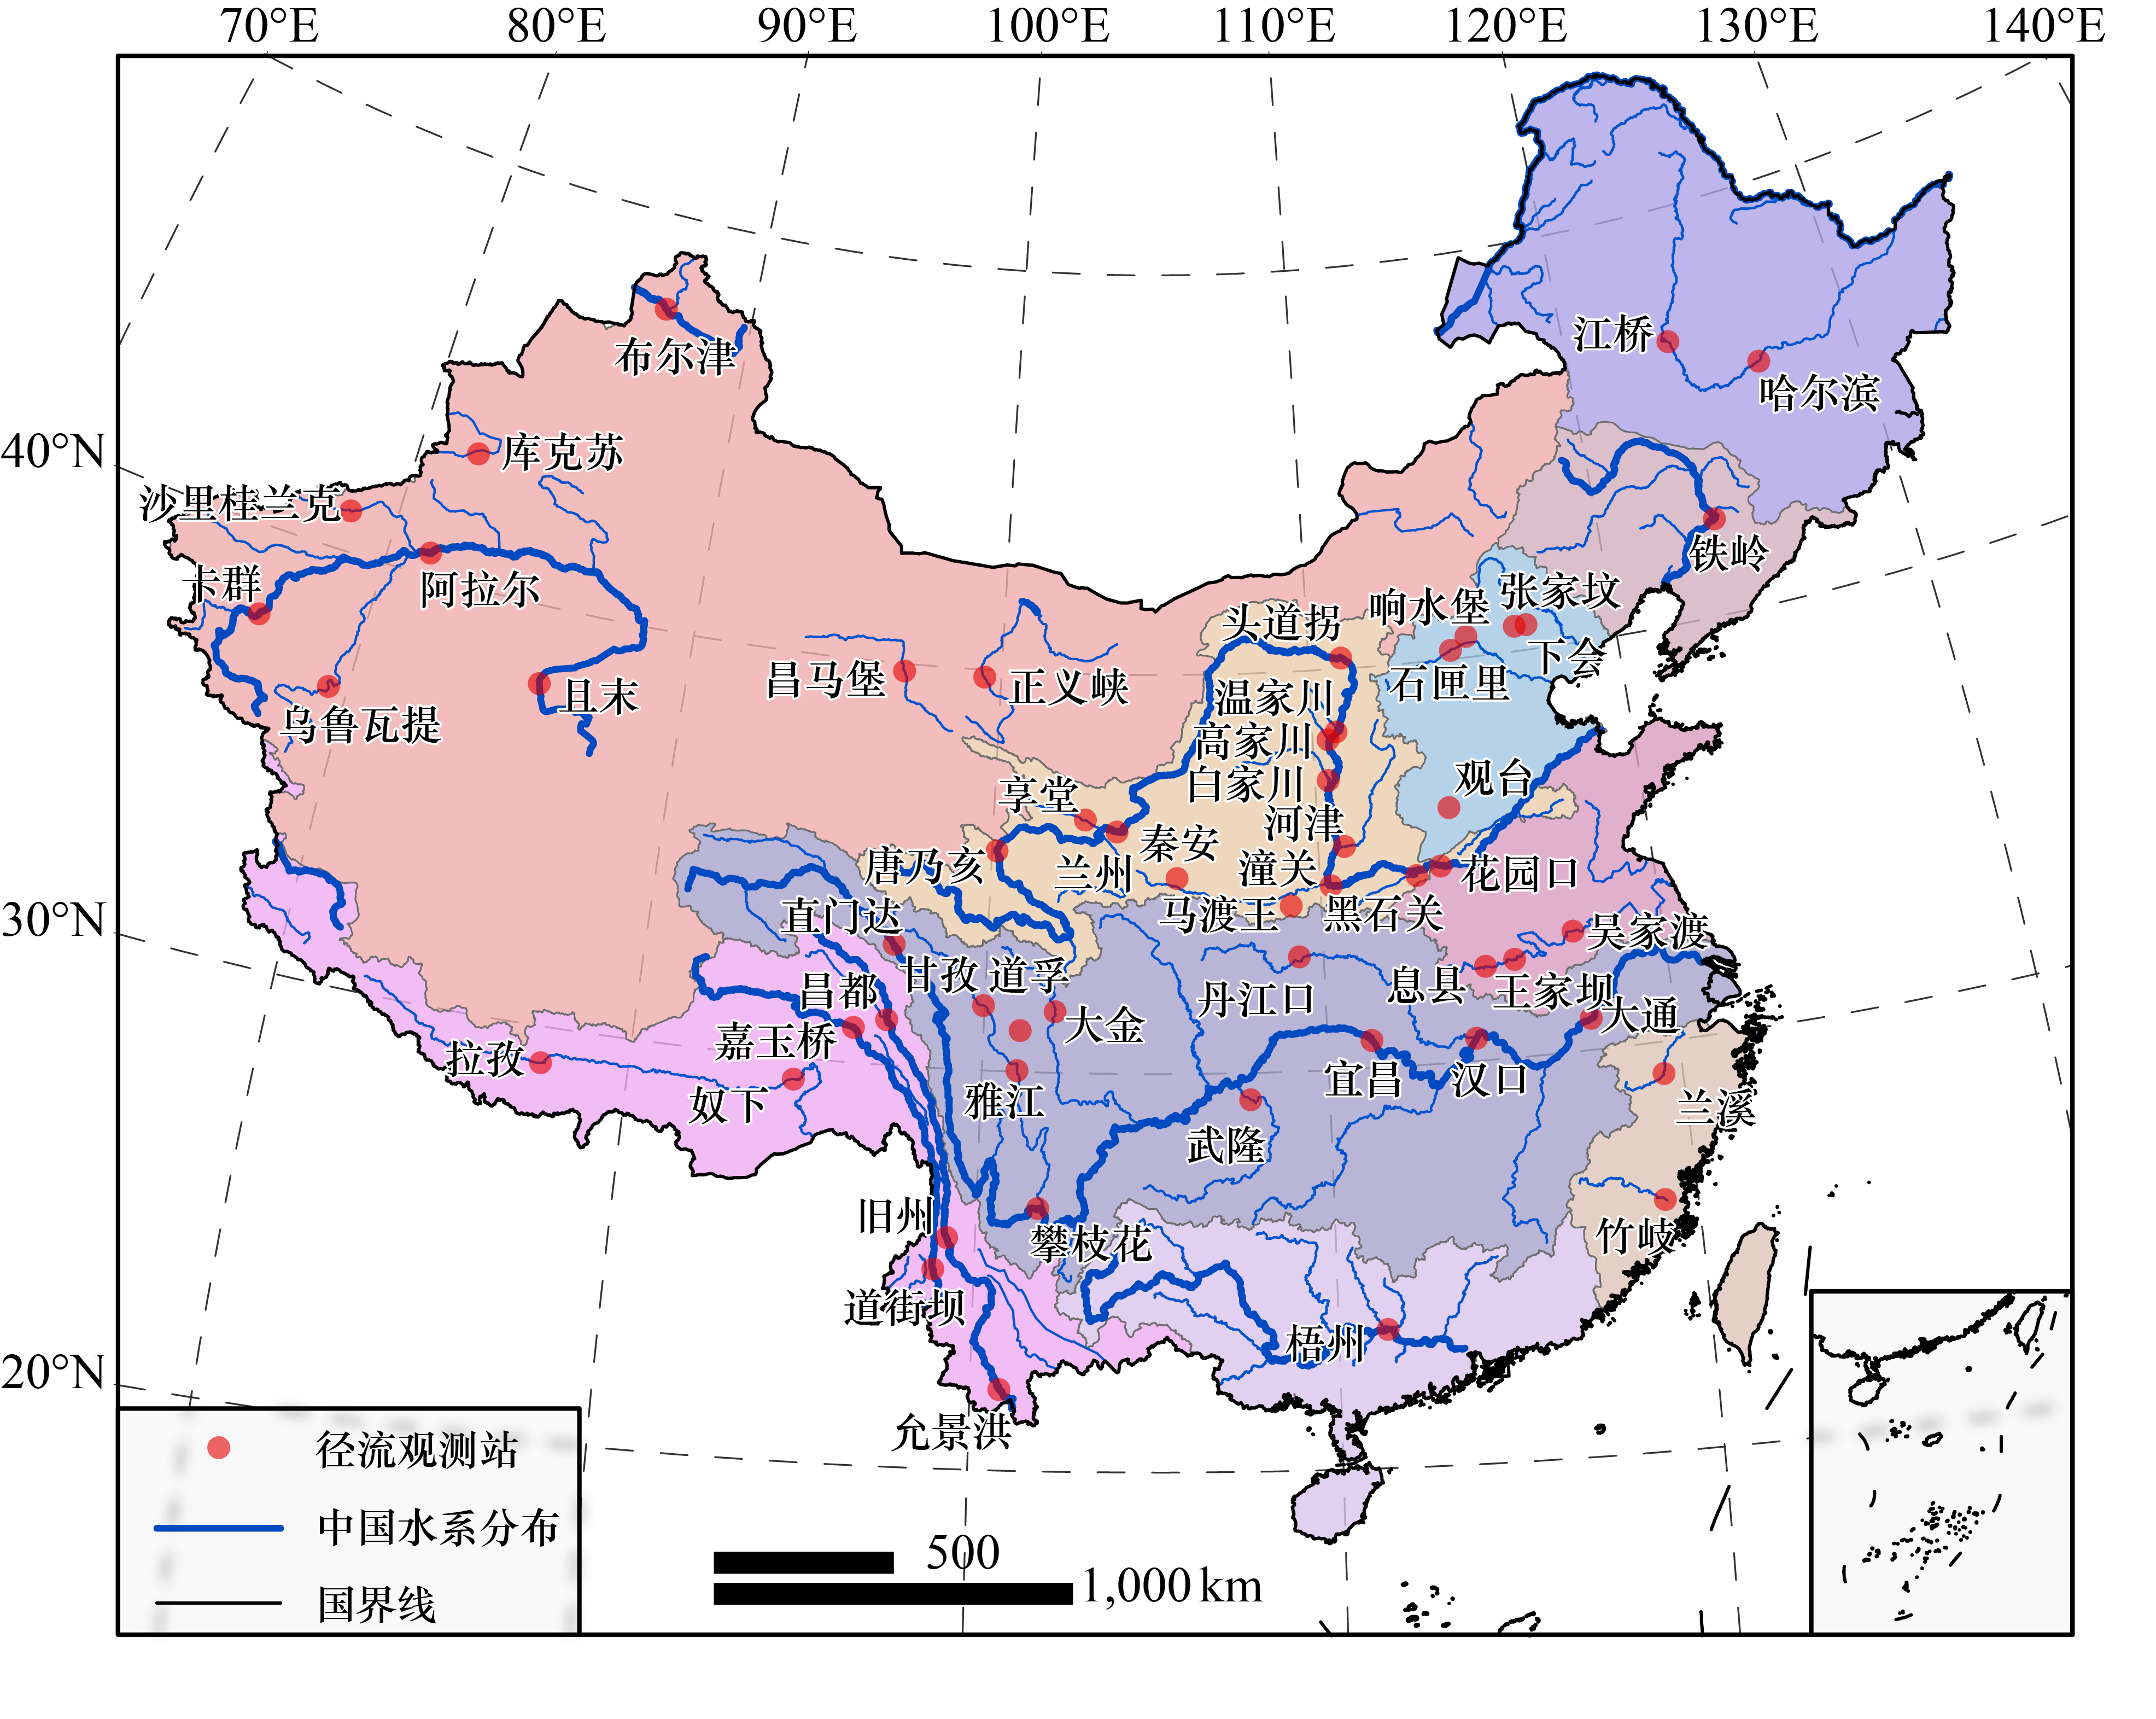
\includegraphics[width=0.85\textwidth]{figures/chap2/China_Stations.jpg}
	\bicaption{中国径流观测站位置图}{Location of Chinese streamflow gauging stations}\label{fig:All_China_Stations}
\end{figure}

\section{研究数据}

论文研究使用的数据包括全球格点尺度上的历史气候学(气温、降水、潜在蒸散发、实际蒸散发、雪水当量)、土壤质地、地形、植被覆盖、径流观测与重建、气候模式输出以及全球陆地分区数据(基于气候条件和基于地理位置的分区)等。这些数据将用于研究全球水文循环历史演变的时空规律、评估与构建全球水文模型以及探究全球水资源对气候变化的相应。表\ref{tab:data}总结了本研究中使用的数据和来源。

\begin{table}[H]\small	%\small用于控制表格内字体大小为5号字
	\centering
	\bicaption{研究使用的气候学、径流和下垫面数据及其来源}{Climatology, runoff and underlying surface data with source used in the research} \label{tab:data}
	\begin{tabular*}{1\textwidth}{@{\extracolsep{\fill}}ccccc}
		\toprule % 第一条线。头部的线
		% 表头
		数据类型 & 数据 & 空间分辨率 & 时间分辨率 & 数据来源 \\
		\midrule % 第二条线,中间的线
		\multirow{8}*{\makecell{历史\\气候条件}} & 降水 & \multirow{3}*{0.5°} & \multirow{3}*{\makecell{1901-2022年\\(月尺度)}} & \multirow{3}*{\makecell{CRU TS v4.07\\气候研究单元时间\\序列数据集}}\\
		~ & 气温 & ~ & ~ & ~ \\
		~ & 潜在蒸散发 & ~ & ~ & ~ \\
		~ & 降水 & \multirow{5}*{0.1°} & \multirow{5}*{\makecell{1951-2024年\\(月尺度)}} & \multirow{5}*{\makecell{ERA5-Land全球气候\\再分析数据集}}\\
		~ & 气温 & ~ & ~ & ~ \\
		~ & 潜在蒸散发 & ~ & ~ & ~ \\
		~ & 实际蒸散发 & ~ & ~ & ~ \\
		~ & 雪水当量 & ~ & ~ & ~ \\
		\midrule % 第二条线,中间的线
		\multirow{7}*{径流} & \multirow{3}*{观测径流} & \multirow{3}*{/} & \multirow{3}*{/} & GRDB全球径流数据库 \\
		~ & ~ & ~ & ~ & \makecell{GSIM全球径流指数\\和元数据存档} \\
		~ & \multirow{2}*{重建径流} & 0.5° & 1902-2014年 & GRUN全球天然径流数据集\\
		~ & ~ & 0.25° & 1961-2018年 & CNRD中国天然径流数据集\\
	    ~ & 径流系数 & \multirow{2}*{0.125°} & \multirow{2}*{/} & \multirow{2}*{全球径流特征数据集(GSCD)} \\
		~ & 基流系数 & ~ & ~ & ~\\
		\midrule % 第二条线,中间的线
		植被特征 & \makecell{归一化植被\\指数NDVI} & 1/12° & 15天 & \makecell{全球模拟和绘图项目(GIMMS)}\\
		\midrule % 第二条线,中间的线
		\multirow{7}*{下垫面} & 高程 & 30米 & / & \makecell{ASTER全球数字高程地图} \\
		~ & 土壤质地 & 30弧度秒 & / & \makecell{联合国粮食及农业组织\\世界土壤数据库(HWSDv1.2)} \\
		~ & 土地利用类型 & 1千米 & / & \makecell{马里兰大学(UMD)\\土地利用数据集} \\
		~ & 流向 & 0.5° & / & \makecell{国际卫星陆地表面气候学\\计划II(ISLSCP II)河流路由数据} \\
		\bottomrule % 第三条线,底部的线
	\end{tabular*}%
\end{table}

\subsection{历史气候再分析数据}

气候研究单元时间序列数据集(Climatic Research Unit Time Series,CRU TS)是英国国家大气科学中心(UK National Centre for Atmospheric Science,NCAS)及其合作者开发的全球历史气候格点再分析数据集(\href{https://crudata.uea.ac.uk/cru/data/hrg/cru_ts_4.07/}{https://crudata.uea.ac.uk/cru/data/hrg/cru\_ts\_ 4.07/},最后访问时间:2024年8月2日)\cite{harrisVersionCRUTS2020}。数据集收集广泛的气象站点观测网络的每月气候数据,有10种变量,分别是近地表气温(最高、最低、平均和昼夜温差)、降水量(总降水量、降水天数)、湿度(蒸汽压)、潜在蒸散发、云量、霜天数等,通过角距离加权(Angular-Distance Weighting,ADW)算法进行插值,以0.5°×0.5°经纬度网格覆盖全球除南极洲以外的世界所有陆地区域,并且每年进行一次更新,目前的数据序列可以覆盖从1901至2022年,是目前可获得的最长数据序列的历史气候再分析数据集。\par

ERA5-Land是欧洲中期天气预报中心(European Centre for Medium-Range Weather Forecasts,ECMWF)在欧盟委员会哥白尼气候变化服务(Copernicus Climate Change Service,C3S)的框架内开发的第五代全球气候再分析数据集(\href{https://cds.climate.copernicus.eu/cdsapp#!/dataset/reanalysis-era5-land-monthly-means?tab=overview}{https://cds.climate.cop ernicus.eu/cdsapp\#!/dataset/reanalysis-era5-land-monthly-means?tab=overview},最后访问时间:2024年8月2日)\cite{hersbachERA5GlobalReanalysis2020,munoz-sabaterERA5LandStateoftheartGlobal2021}。与ERA5相比,它以更高的分辨率提供了数十年来陆地变量演变的一致视图。ERA5-Land是通过气候强迫驱动ECMWF ERA5物理模型的陆地部分进行重新计算而生成的,并进行了热力学近地表状态的高程校正。模型利用物理定律将模型数据与来自世界各地的观测结果相结合,形成一个全球水和能源演变的完整且一致的数据集。数据集包括了多种气象要素,如气温、降水、潜在蒸散发、实际蒸散发、雪水当量等,以0.1°×0.1°经纬度网格覆盖全球陆地区域,时间分辨率为小时和月,时间范围从1951年至今。ERA5-Land以其高时空分辨率支持设计水资源、土地和环境管理的各种应用。\par

\subsection{网格径流数据}

在分布式水文模型的应用过程中,当仅使用出口站点的径流数据时,集水区范围内的空间异质性被均化处理,无法提供空间模式信息。相较于站点观测径流数据,网格化数据以其相对统一的空间分辨率、对非自然流域描述的高自由度,被广泛应用于大尺度研究中。\par

\subsubsection{全球网格径流数据}

全球格点径流数据集(Global Gridded Runoff Dataset,GRUN)是一个基于观测径流数据的全球网格化重建径流数据集(\href{https://figshare.com/articles/dataset/GRUN_Global_Runoff_Reconstruction/9228176}{https://figshare.com/articles/dataset/GRUN\_Global \_Runoff\_Reconstruction/9228176},最后访问时间:2024年8月2日),由Ghiggi等人开发\cite{ghiggiGRUNObservationbasedGlobal2019, ghiggiGRUNENSEMBLEMultiForcing2021}。原位观测径流被用于训练机器学习算法,根据大气再分析中的前期气温和降水来预测月径流,并进行交叉验证评估,并与大型河流的一组独立的径流观测数据进行比较。与13个最先进的全球水文模型径流模拟的集合相比,GRUN具有更好的平均一致性和更低的不确定性。GRUN数据集提供了全球0.5°×0.5°经纬度网格的月尺度径流数据,时间范围为1902-2014年。该数据集被广泛应用于全球淡水动态、年际变化、干旱传播以及径流对大气遥相关的响应等方面的研究。\par

\subsubsection{全球网格径流特征数据}

全球径流特征图(Global Streamflow Characteristics Dataset,GSCD)包含17种径流特征的全球地图,例如基流指数、径流系数和流量百分位数,提供有关整个陆地表面(包括未测量区域)径流行为的信息\cite{beckGlobalPatternsBase2013, beckGlobalMapsStreamflow2015},通过GloH2O发布(\href{https://www.gloh2o.org/gscd/}{https://www.gloh2o.org/gscd/},最后访问时间:2024年8月2日)。利用全球超过3000个中小型流域(集水区面积介于10-10000千米\textsuperscript2之间)观测到的日径流资料训练集合神经网络,以根据流域的气候和地貌特征估计径流特征参数。经过训练的集合神经网络被应用在整个无冰陆面上,以生成全球0.125°×0.125°网格上的径流特征地图。

\subsubsection{中国网格径流数据}

中国天然径流数据集(China Natural Runoff Dataset,CNRD)是由北京师范大学Gou等\cite{gouCNRDV1HighQuality2021, gouSensitivityAnalysisBased2020, gouSeasonalityImpactFactor2022, GouJiaoJiaoJiYuVICDeZhongGuoTianRanJingLiuGuSuanYuPingJie2021}人开发的覆盖中国大陆的质量控制的历史网格化天然径流重建数据集(\href{https://figshare.com/articles/dataset/CNRDv1_0/13185410}{https:// figshare.com/articles/dataset/CNRDv1\_0/13185410},最后访问时间:2024年8月2日)。数据集提供了1961-2018年期间中国的日、月和年0.25°×0.25°径流估算。CNRD使用可变下渗容量模型(Variable Infiltration Capacity,VIC)生成,利用超过200个自然或接近自然的标准集水区训练模型,并结合参数敏感性分析、优化和区域化框架以提高产品稳健性。CNRD是中国第一个使用不确定性框架估算网格化天然径流的数据集,为大尺度径流估算提供了重要的数据和方法参考。\par

\begin{figure}[H]
	\centering
	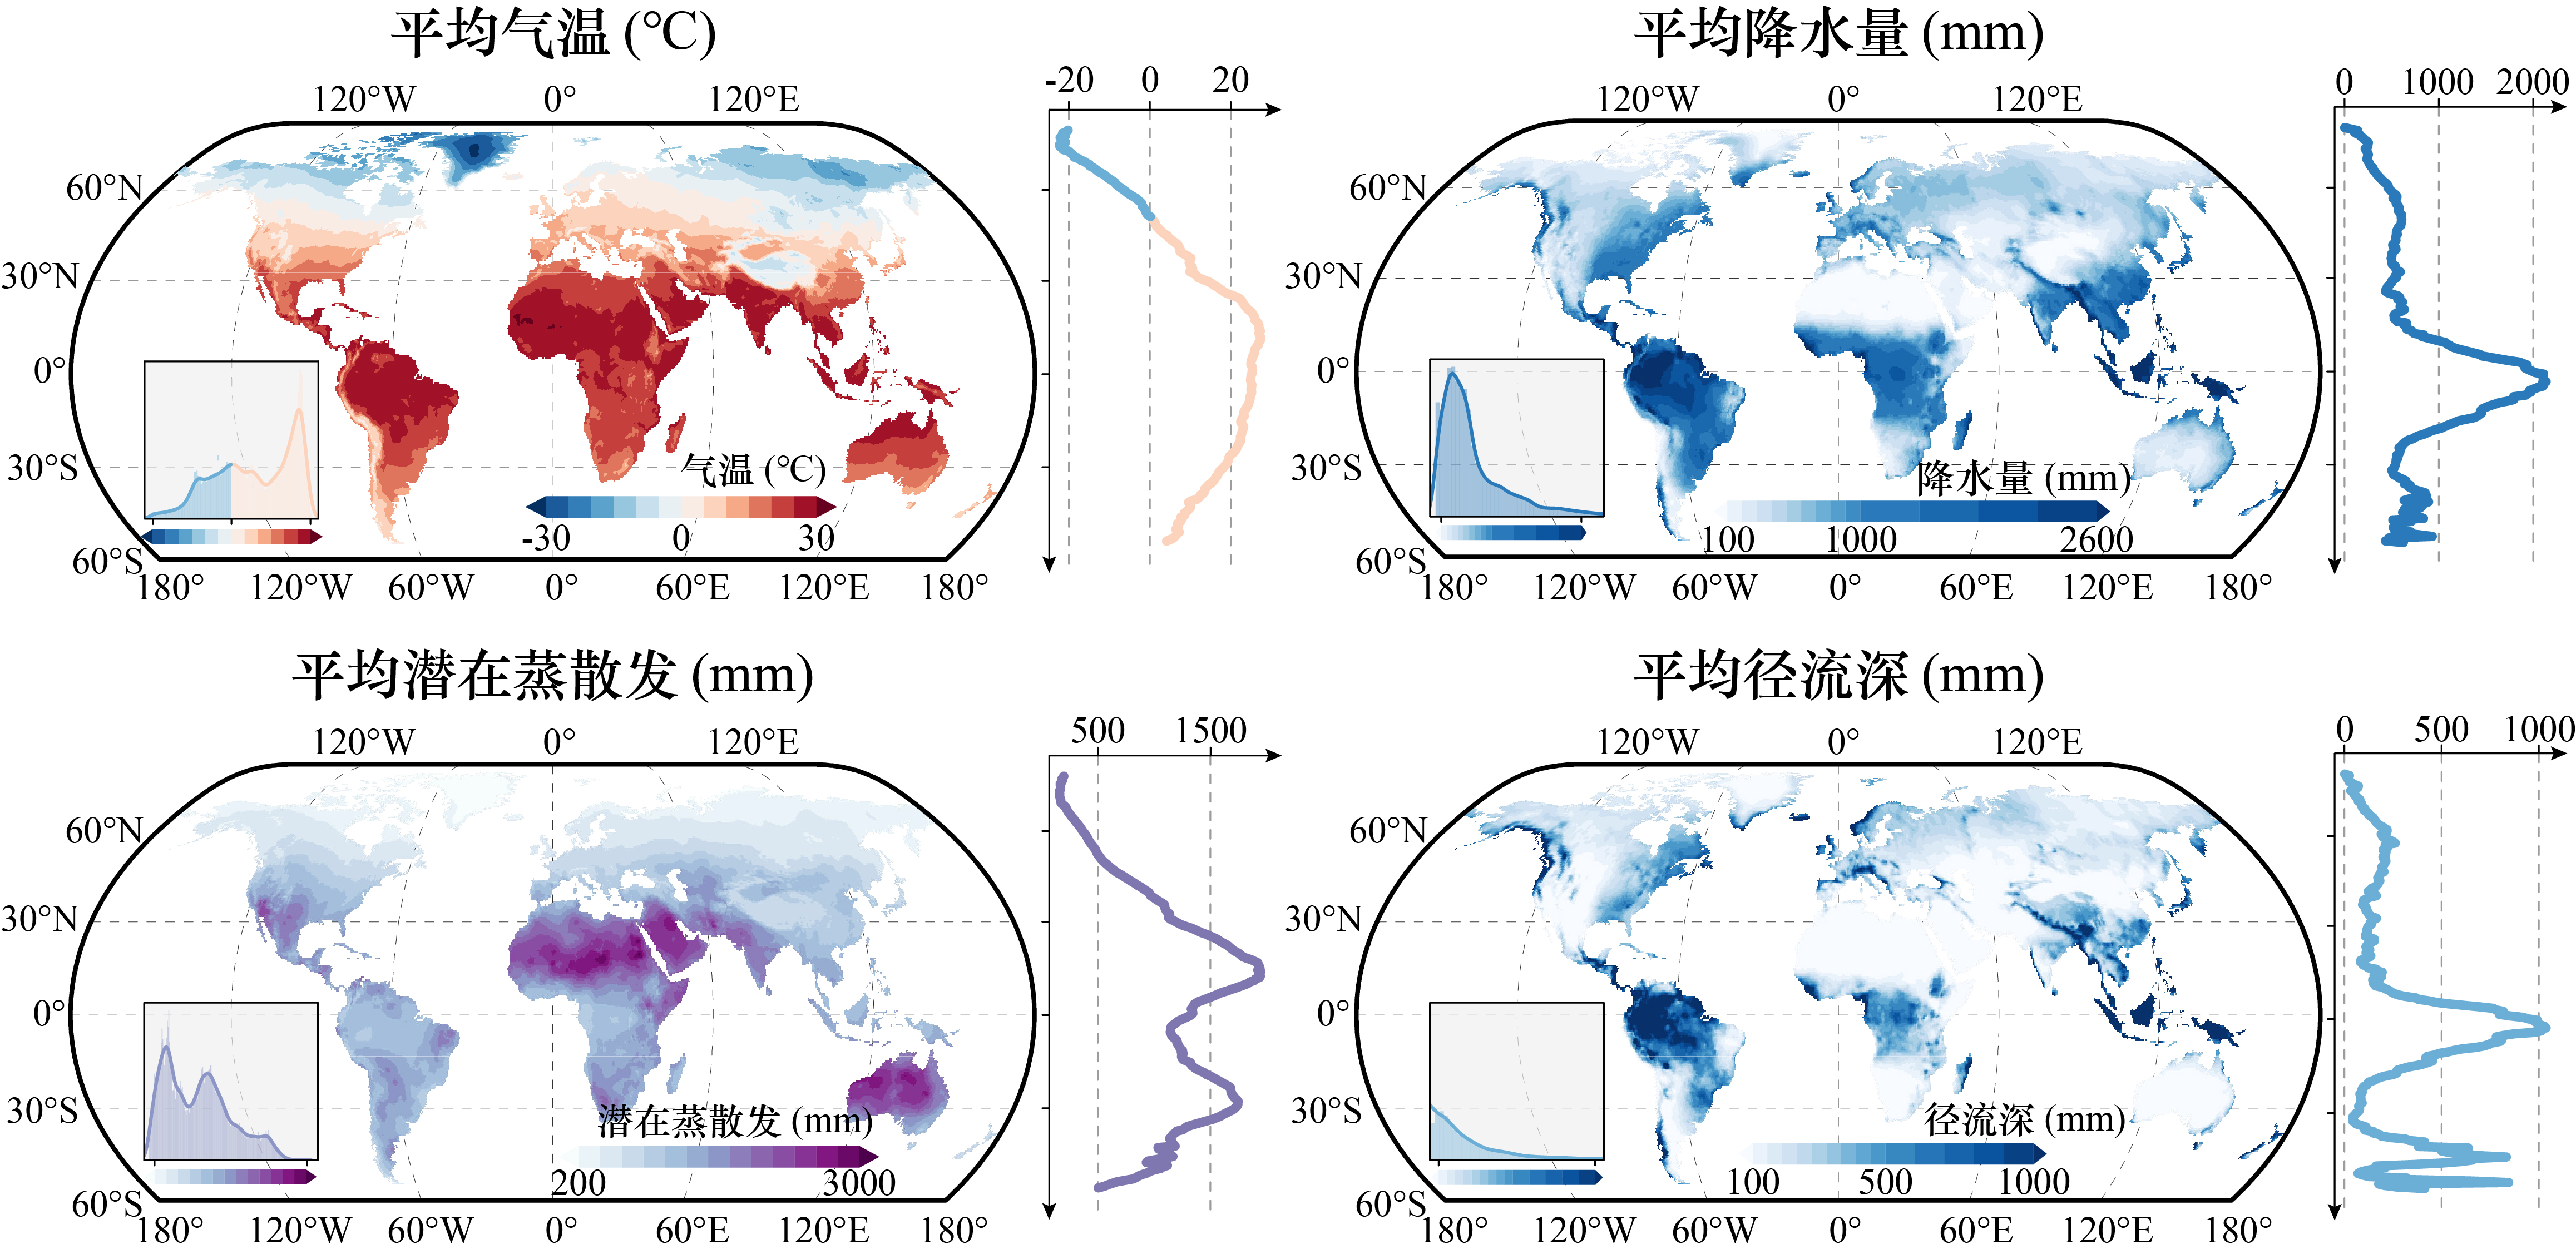
\includegraphics[width=1\textwidth]{figures/chap2/Global_Ave_Climatic.jpg}
	\bicaption{全球历史气候与径流数据}{Global historical climatic and runoff data}\label{fig:Global_Climatic_Data}
\end{figure}

\subsection{下垫面数据}

本论文使用的下垫面数据包括高程、土壤质地、流向和植被覆盖等。下垫面条件的空间异质性对流域水循环过程有重要的影响,因此需要在水文模型中考虑下垫面条件的时空分异模式。

\subsubsection{高程数据}

数字高程模型(Digital Elevation Model,DEM)是对地表地形的数字表示。本研究采用的DEM数据来源于日本经济产业省(Ministry of Economy,Trade,and Industry of Japan,METI)与美国国家航空航天局(United States National Aeronautics and Space AdministrationNASA)联合发布的先进星载热发射和反射辐射计(Advanced Spaceborne Thermal Emission and Reflection Radiometer,ASTER)全球数字高程模型第3版(GDEM v003)。ASTER GDEM是通过ASTER传感器在2000年至2011年间的卫星影像数据生成的,覆盖范围从北纬83°到南纬83°,涵盖了地球99\%的陆地面积,空间分辨率为30米,并且具有1°×1°的图块。该DEM数据广泛应用于地理信息系统、环境监测、自然灾害评估、地质研究等领域。数据在NASA的数据网站Earthdata(\href{https://search.earthdata.nasa.gov/search/}{https://search.earthdata.nasa.gov/search/},最后访问时间:2024年8月2日)上提供公开下载。

\subsubsection{土壤质地数据}

土壤质地是对土壤颗粒组成的描述。联合国粮食及农业组织(Food and Algriculture Organization,FAO)联合国际应用系统分析研究所(International Institute for Applied Systems Analysis,IIASA)、中国科学院南京土壤研究所(Institute of Soil Science,Chinese Academy of Sciences,ISSCAS)和欧盟委员会联合研究中心(Joint Research Centre of the European Commission,JRC)发布了全球30弧度秒分辨率的世界土壤数据库(Harmonized World Soil Database,HWSD v1.2)。该数据库包含超过15,000个不同的土壤测绘单元,综合了现有世界各区域和国家更新的土壤信息,并进行统一标准的分类,使用标准化结构将属性数据与栅格地图联系起来。土壤特征参数主要包括有机碳,pH值,土壤深度,土壤类型,砂土、壤土、粘土三种组分含量,土壤质地等。其中土壤质地由土壤三种组分含量通过美国农业部(US Department of Agriculture,USDA)的土壤质地分类三角(Soil Texture Classification Triangle)进行划分,分为砂土、壤土等12种类型\cite{moreno-marotoEvaluationUSDASoil2022}。数据在FAO网站上(\href{https://www.fao.org/soils-portal/data-hub/soil-maps-and-databases/harmonized-world-soil-database-v12/en/}{https://www.fao.org/soils-portal/data-hub/soil-maps-and-databases/harmonized-world-soil-database-v12/en/},最后访问时间:2024年8月2日)提供公开下载。

\subsubsection{流向数据}

模拟拓扑网络(Simulated Topological Network,STN-30p)为分布式水文模型构建提供了全球河流系统的精确表示,包括全球0.5°网格上的流向、河道长度、河道等级等信息。STN-30p数据集为每个陆地网格单元分配了8个可能的流向之一,来表明陆地之间的潜在连通性。数据集由国际卫星陆地表面气候学计划II(International Satellite Land Surface Climatology Project II,ISLSCP II)发布(\href{https://daac.ornl.gov/cgi-bin/dsviewer.pl?ds_id=1005}{https://daac.ornl.gov/cgi-bin/dsviewer.pl?ds\_id=1005},最后访问时间:2024年8月2日)。

\subsubsection{植被覆盖数据}

流域植被覆盖与降水冠层截留、植被蒸腾作用密切相关。归一化植被指数(NormalizedDifference Vegetation Index, NDVI)是植被冠层绿叶中叶绿素吸收的光合有效辐射的辐射测量,是反映流域植被特征的重要指标。NDVI值的范围为1.0到-1.0。贫瘠的岩石、沙地或积雪区域通常显示非常低的NDVI值(0.1或更低)。稀疏的植被(例如灌木和草地)或衰老的作物可能导致中等的NDVI值(大约0.2到0.5)。高NDVI值(大约0.6到0.9)对应于茂密的植被,例如温带和热带森林中的植被或处于生长高峰期的作物。\par
本研究使用的NDVI数据来自全球模拟和绘图项目(Global Inventory Modeling and Mapping Studies,GIMMS)发布的15天间隔的1/12°分辨率的NDVI数据集(\href{https://www.ncei.noaa.gov/data/land-normalized-difference-vegetation-index/access/}{https://www.ncei.noaa.gov/data/land-normalized-difference-vegetation-index/access/},最后访问时间:2024年8月2日)。该数据集基于NASA的先进非扫描辐射计(Advanced Very High Resolution Radiometer,AVHRR)传感器,经过辐射校正和坐标转换,并消除由于轨道偏移等偏差后发布,覆盖了1981年7月至今的全球陆地表面,提供了全球植被覆盖的时空变化信息。

\begin{figure}[H]
	\centering
	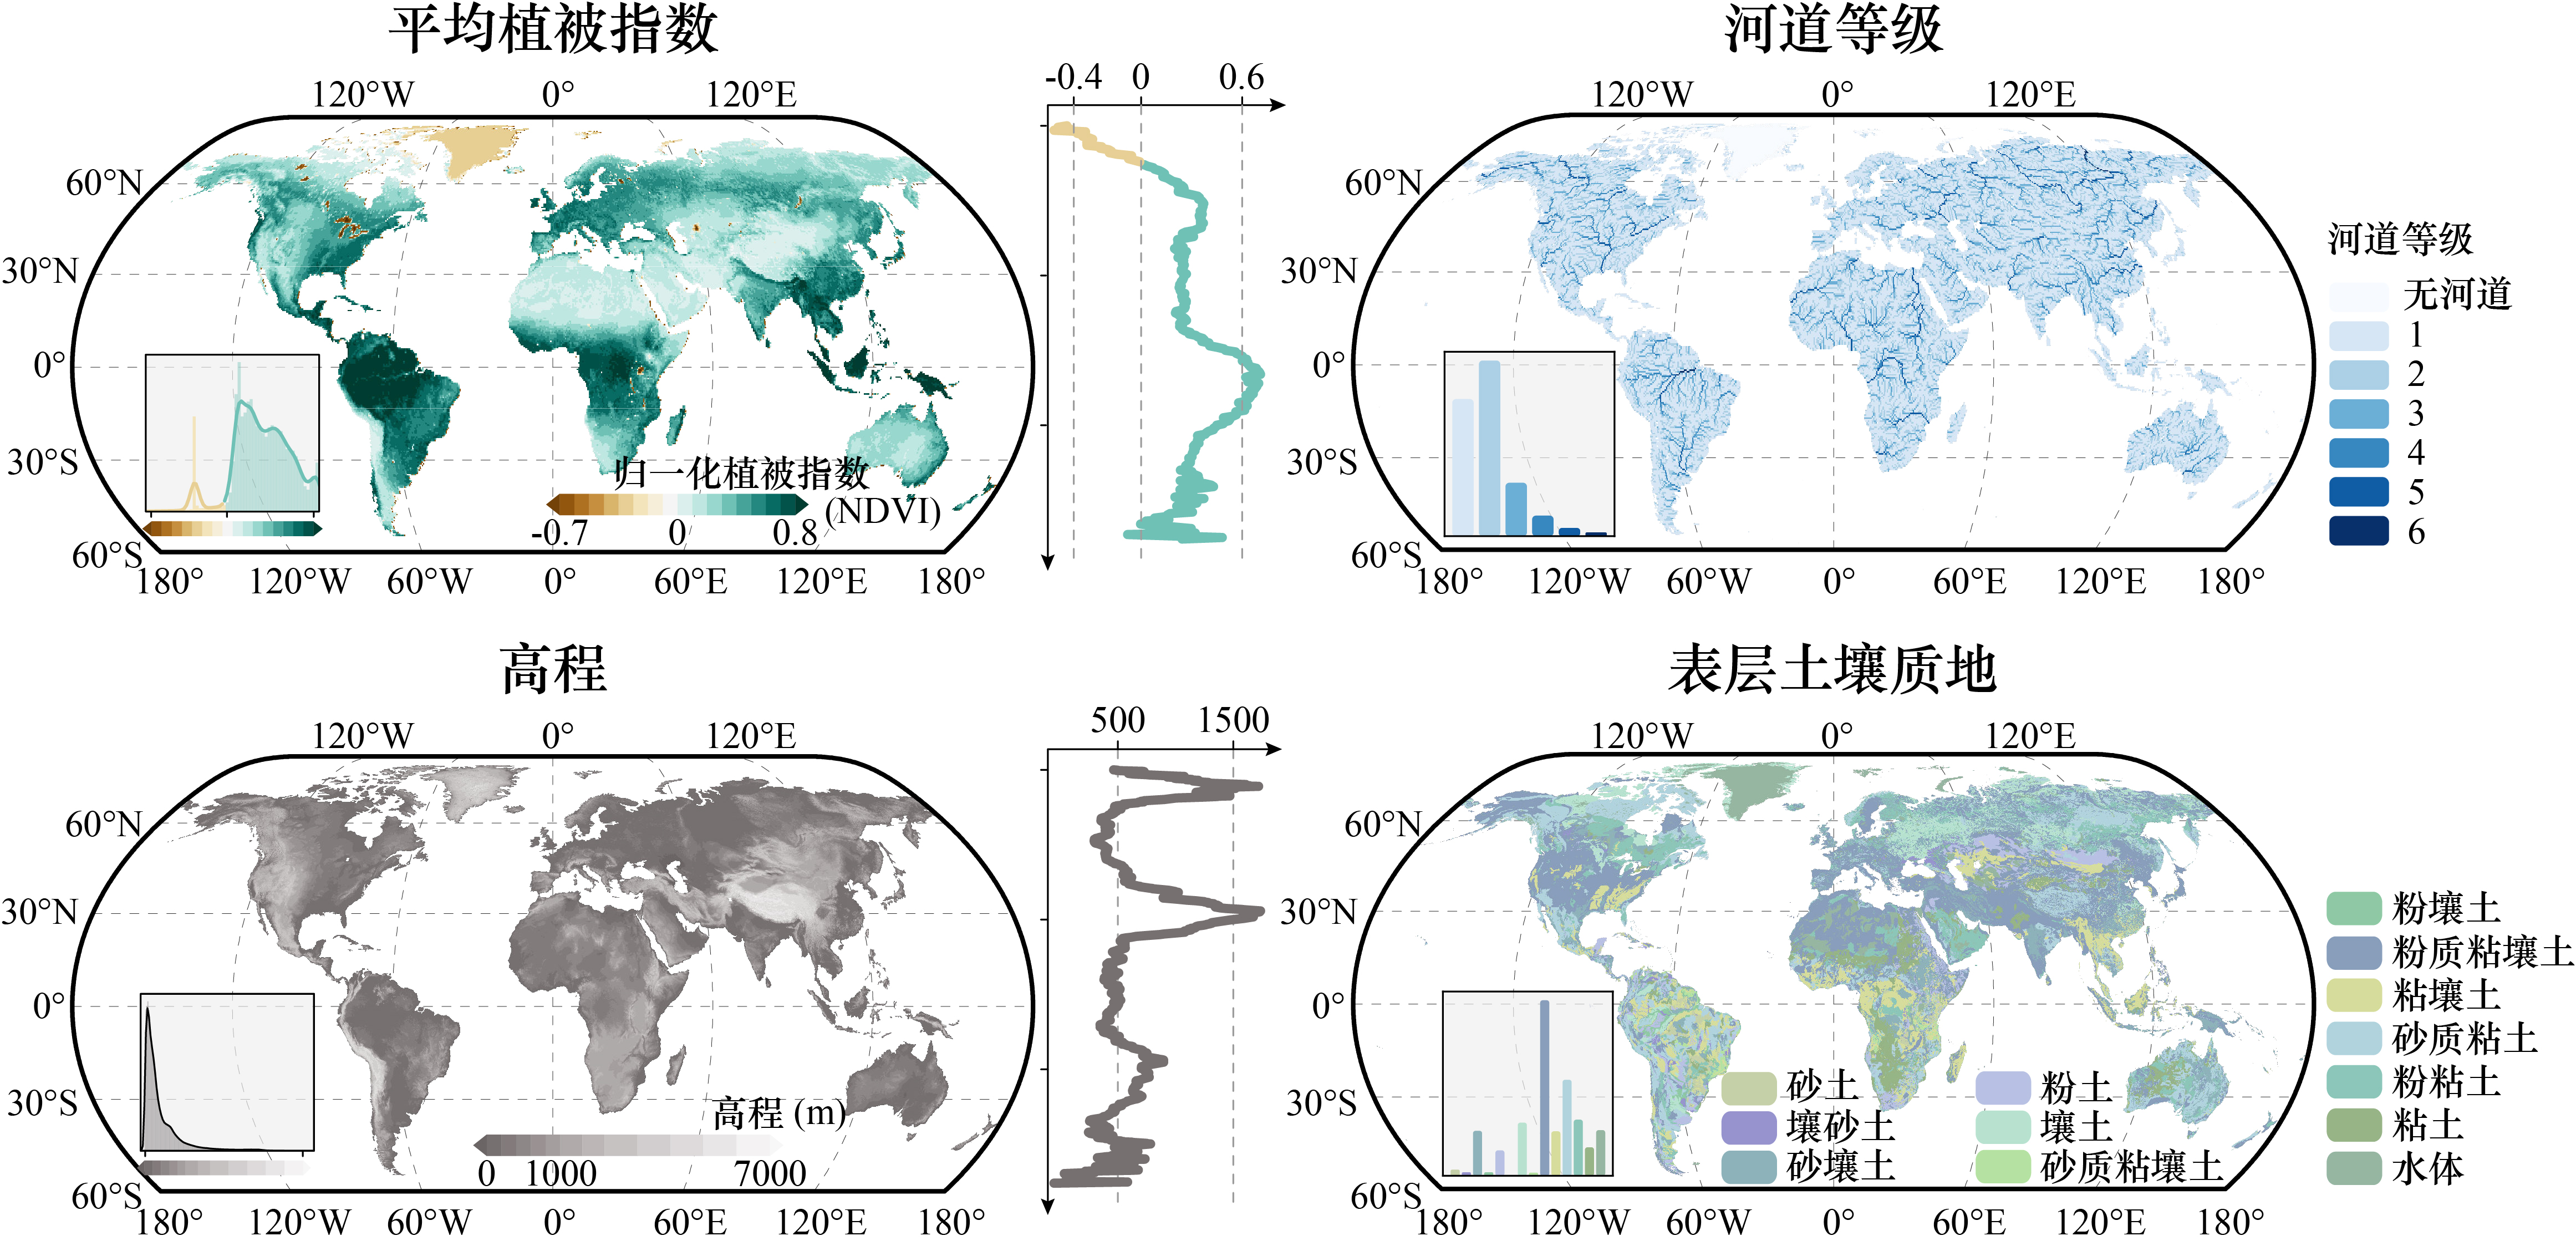
\includegraphics[width=1\textwidth]{figures/chap2/Global_Underlying.jpg}
	\bicaption{全球陆地下垫面数据}{Underlying surface data of global land}\label{fig:Global_Underlying_Data}
\end{figure}

\subsection{气候模式数据}

全球气候模型(Global Climate Model,GCM)是一种用于模拟全球气候系统的数值模型,是研究全球气候变化的重要工具。GCM利用一系列的数学公式来描绘气候系统的各个主要组成部分,包括大气、海洋、冻土以及地表和海洋表面的生物地理过程。世界气候研究计划组织(World Climate Research Programme,WCRP)自20世纪90年代起组织了一系列的耦合模式比较计划(Coupled Model Intercomparison Project,CMIP),目前已经发展到第六阶段(CMIP6)。CMIP6的目标是为全球气候变化研究提供最新的全球气候模型模拟数据,以评估全球气候模型的性能,分析全球气候变化的趋势\cite{ZhouTianJunDiLiuCiGuoJiOuHeMoShiBiJiaoJiHuaCMIP6PingShu2019}。作为CMIP6的一部分,每个模型都提供了1850-2014的历史气候情况模拟及2015-2100年的未来气候预测\cite{ningWetterTrendSource2024}。\par
本研究使用的气候模型数据来自共享社会路径(Shared Socioeconomic Pathways,SSP)下的四种情景,分别是绿色发展路径(SSP1-2.6)、中间路径(SSP2-4.5),区域对抗路径(SSP3-7.0)和化石燃料路径(SSP5-8.5)试验下的全球月尺度气温、降水和太阳辐射强度输出,采用了来自CMIP6的17种GCM输出数据(\href{https://esgf-node.ipsl.upmc.fr/search/cmip6-ipsl/}{https://esgf-node.ipsl.upmc.fr/search/cmip6-ipsl/})。表\ref{tab:gcmdata}汇总了所选GCM模型的具体信息。

\begin{table}[H]\small	%\small用于控制表格内字体大小为5号字
	\centering
	\bicaption{本研究中使用的未来气候模式信息}{Global climate models used in the research} \label{tab:gcmdata}
	\begin{tabular*}{0.9\textwidth}{@{\extracolsep{\fill}}cccc}
		\toprule % 第一条线。头部的线
		% 表头
		序号 & 气候模式 & 研发机构/地区 & 空间分辨率 \\
		\midrule % 第二条线,中间的线
		1 & ACCESS-CM2 & \multirow{2}*{CSIRO/澳大利亚} & \multirow{2}*{1.875°×1.25°} \\
        2 & ACCESS-ESM1-5 & ~ & ~ \\
        3 & BCC-CSM2-MR & BCC/中国 & 1.125°×1.125° \\
        4 & CanESM5 & CCCma/加拿大 & 2.8125°×2.8125° \\
        5 & CAS-ESM2-0 & CAS/中国 & 1°×1° \\
        6 & EC-Earth3 & \multirow{2}*{\makecell{EC-Earth-Consortium\\瑞典}} & \multirow{2}*{0.703°×0.703°} \\
        7 & EC-Earth3-Veg-LR & ~ & ~ \\
        8 & FIO-ESM-2-0 & CAS/中国 & 1°×1° \\
        9 & GFDL-CM4 & NOAA-GFDL/美国 & 1°×1.25° \\
        10 & INM-CM4-8 & \multirow{2}*{INM/俄罗斯} & \multirow{2}*{2°×1.5°} \\
        11 & INM-CM5-0 & ~ & ~ \\
        12 & IPSL-CM6A-LR & IPSL/法国 & 1.5°×1.25° \\
        13 & MIROC6 & MIROC/日本 & 1.40625°×1.40625° \\
        14 & MPI-ESM1-2-HR & \multirow{2}*{MPI-M/德国} & 0.9375°×0.9375° \\
        15 & MPI-ESM1-2-LR & ~ & 1.875°×1.8625° \\
        16 & MRI-ESM2-0 & MRI/日本 & 1.125°×1.125° \\
        17 & NESM3 & NUIST/中国 & 1.875°×1.865° \\
		\bottomrule % 第三条线,底部的线
	\end{tabular*}%
\end{table}

\subsection{全球分区数据}

本研究使用不同类型的全球陆地分区数据评估全球历史水文气候条件演变特征以及各种模型的性能规律。

\subsubsection{全球气候分区数据}

柯本气候分区是目前最常用的气候分类方法之一,主要根据当地气候条件和植被类型对世界各地的气候区进行分类\cite{peelUpdatedWorldMap2007,beckPresentFutureKoppenGeiger2018}。首先根据全球气候将陆地划分为五个主气候带,分别是赤道带(A,最低气温高于18℃),干旱带(B,年降水量低于10倍降水阈值),暖温带(C,最热月气温高于10℃且最冷月气温介于0-18℃之间),亚寒带(D,最热月气温高于10℃且最冷月气温低于0℃)和极地带(E,最热月气温低于10℃)。之后在每个大类分区中,再根据降水或气温的季节性特征,进行细分类目的识别。全球根据气候条件被划分为30个气候分区,如图\ref{fig:Global_Region_Data}所示。

\subsubsection{IPCC陆地参考分区数据}

为了更好地评估和描述在次大陆尺度的历史趋势和未来气候变化预测,国际气候变化专门委员会(Intergovernmental Panel on Climate Change,IPCC)更新了全球陆地参考分区数据\cite{iturbideUpdateIPCCClimate2020},将全球陆地划分为61个区域(陆地46个,海洋15个),使其更好的代表了一致的区域气候特征。

\begin{figure}[H]
	\centering
	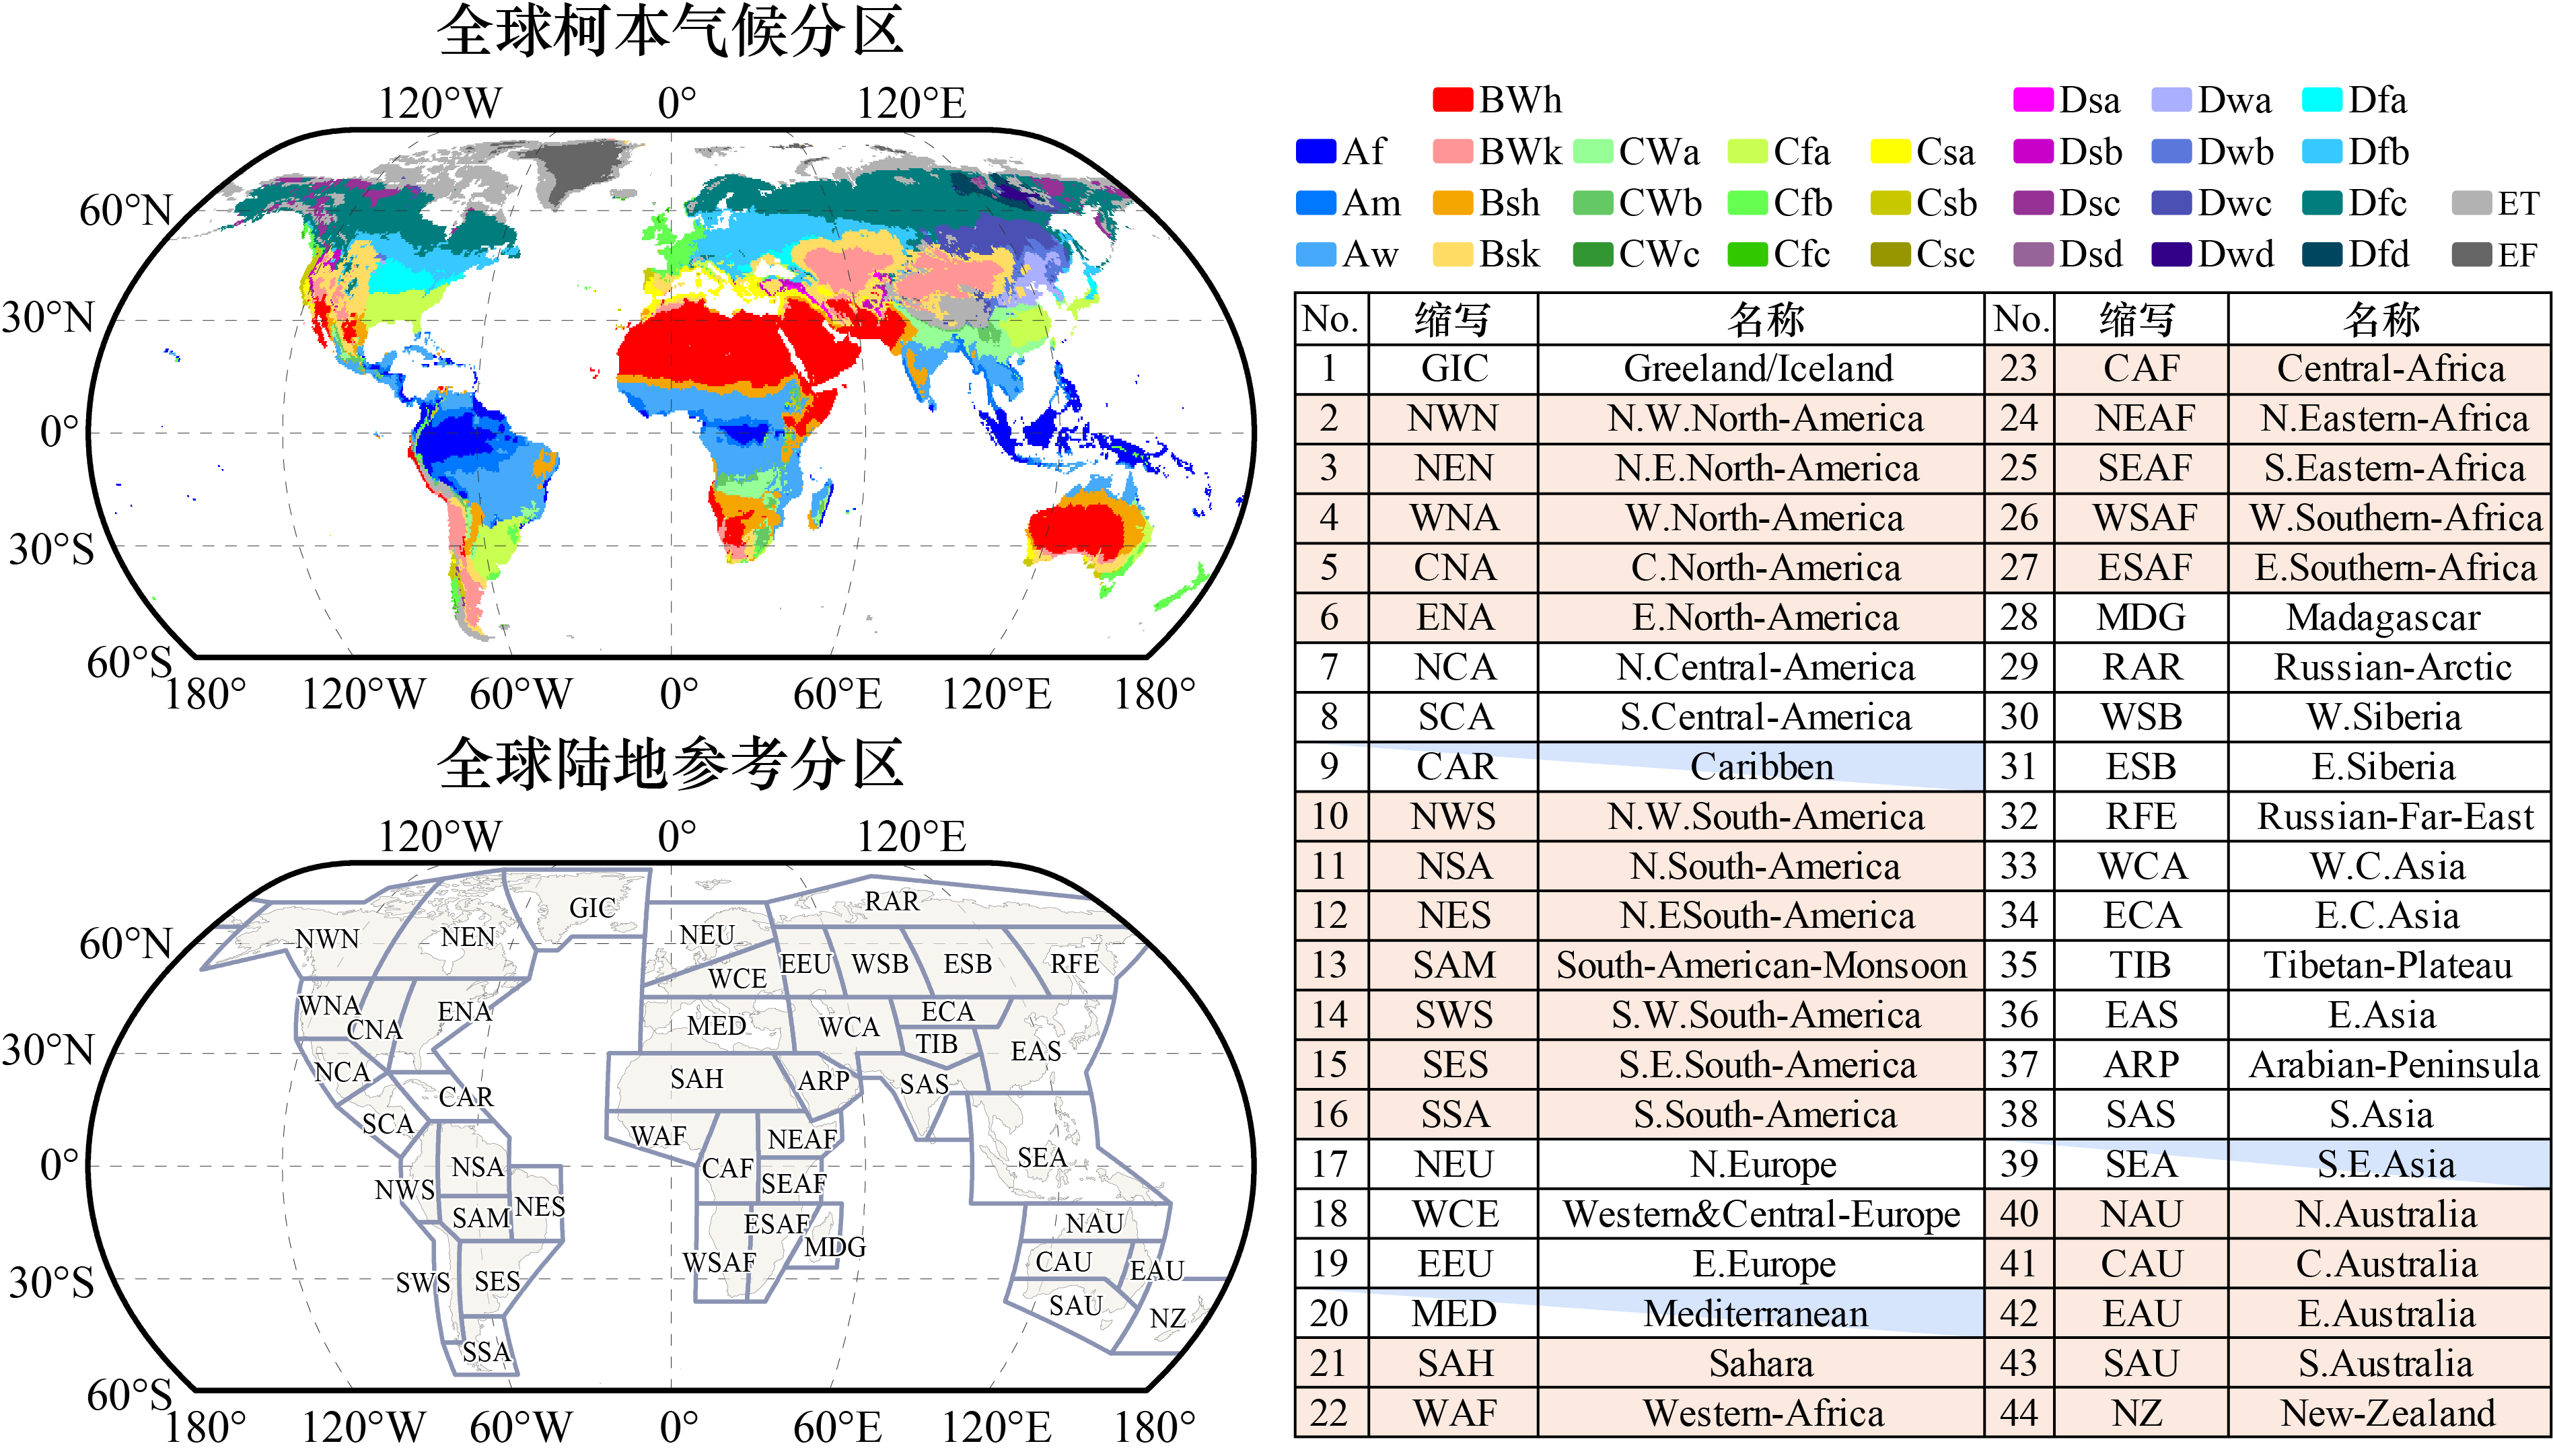
\includegraphics[width=0.9\textwidth]{figures/chap2/Global_Region.jpg}
	\bicaption{全球陆地分区数据}{Köppen and reference region data in global land}\label{fig:Global_Region_Data}
\end{figure}

\clearpage